\section{Domain knowledge}
    \subsection{Biology}
        \subsubsection{Cell line development process}
        General theory behind the cell line development process. Starting from what proteins are. How cells are developed. Difficulties of the cell line development process and timelines.
        \subsubsection{Project specifications of cell line development for Merck KgaA}
        Description of my project, why is it useful, what are the processes here. How my neural network can be used for further stability predictions.
    \subsection{Deep learning and machine learning basics}
        Introduction of the notaiton for the dataset, parameters, predictions.
        \subsubsection{Neural networks}
            Convolutional neural network, Autoencoder, embedding, optimizers, regularization, descriptions of how each layer works.
\begin{figure}[htb]
	\begin{center}
		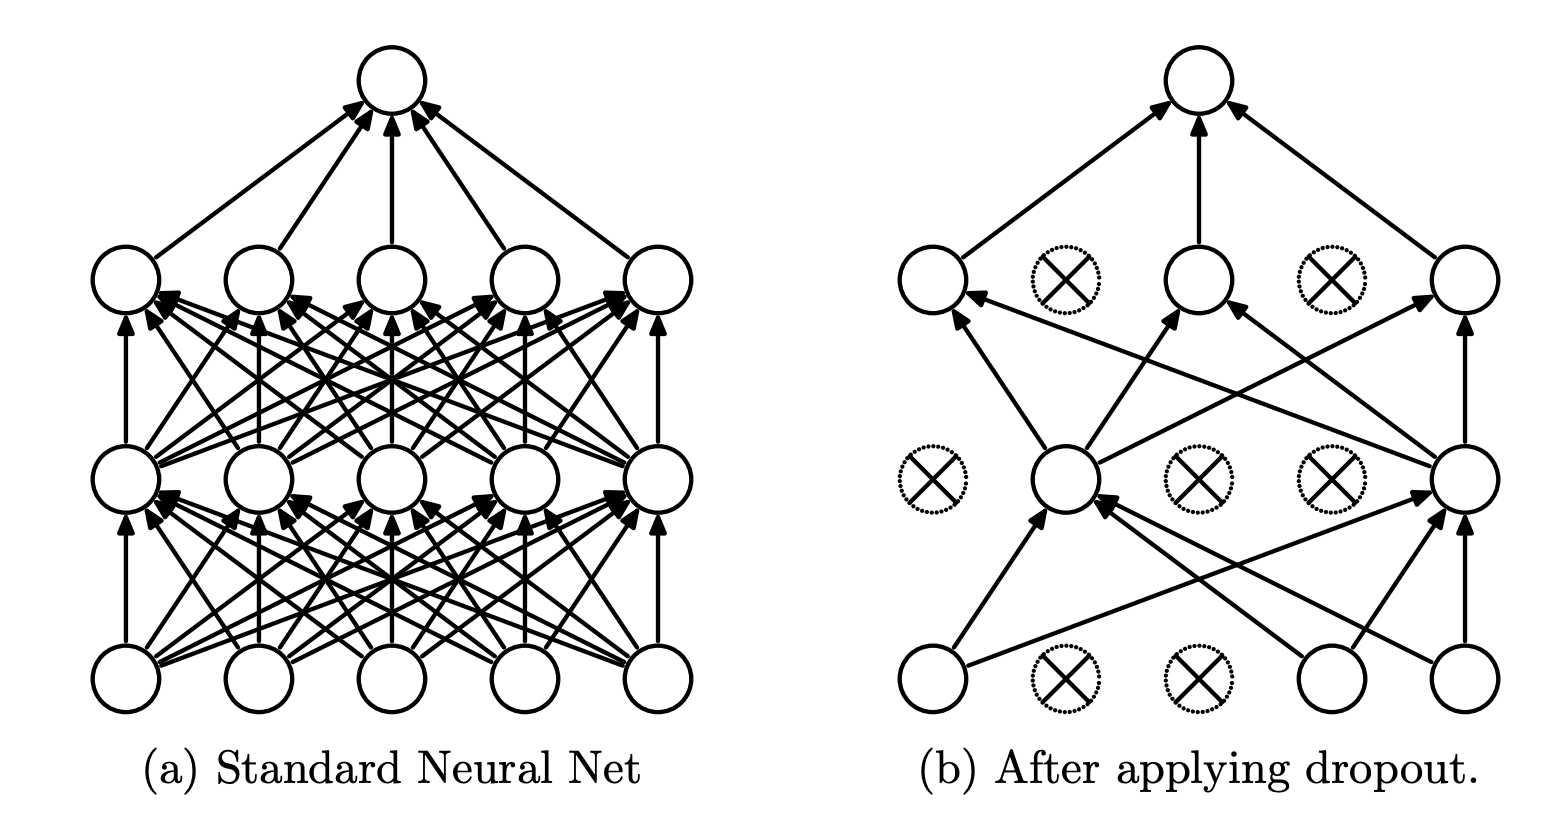
\includegraphics[width=0.8\linewidth]{bilder/dropout.png}
		\caption{Dropout}\label{fig:dropout}
	\end{center}
\end{figure}
        \subsubsection{Clustering}
            Theory of clustering algorithms, DBSCAN, HDBSCAN, PCA
    \subsection{Imaging}
        \subsubsection{Digital imaging}
            How image is stored in memory, which conventions there are (RGB, BGR (conventions are used in corruptions augmentations)).
        \subsubsection{Microscopy imaging}
            \begin{figure}[htb]
                \begin{center}
                    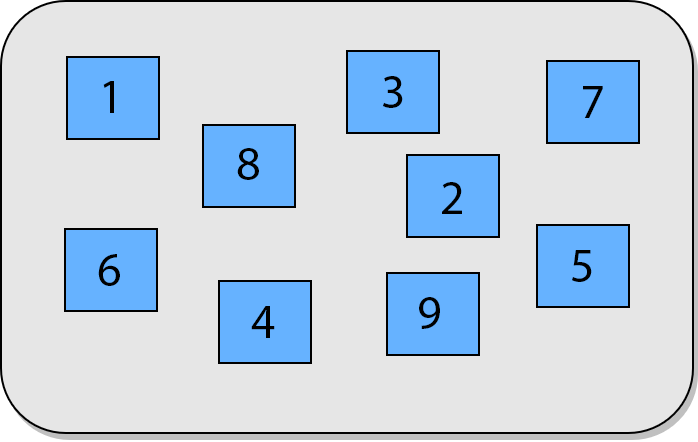
\includegraphics[width=0.5\linewidth]{bilder/dic-random.png}
                    \caption{Way in which photos of the well-plate were taken}\label{fig:random-dic}
                \end{center}
            \end{figure}    
            Which difficulties it may cause (validation loss is lower than train loss)